\section{Описание предметной области}

\subsection{Протокол сериализации Protocol Buffers}

Protocol Buffers ~--~ не зависящий от языка и платформы механизм сериализации структурированных данных, предложенный компанией Google 
как более быстрая и компактная альтернатива текстовому формату XML. Разработчики сообщают \cite{protobuf_doc}, что Protocol Buffers проще, 
компактнее и быстрее, чем XML, поскольку осуществляется передача бинарных данных, оптимизированных под минимальный размер сообщения. 
Формат подходит как для краткосрочного обмена данными по сети, так и для долговременного компактного хранения больших объёмов данных.

Рассмотрим основные преимущества формата.

\subsubsection{} Скорость обработки и компактность сериализованных данных

Protocol Buffers предлагает компактный бинарный формат сериализации данных.
Он обеспечивает высокую степень сжатия, что позволяет экономить пропускную способность сети и место на диске. 
Кроме того, сериализация и десериализация данных в формате Protocol Buffers обрабатываются эффективно и быстро.
В 2010 году бэкенд Twitter перешёл на Protocol Buffers.

По заявлению разработчиков Twitter, база данных, содержащая триллион твитов, в формате XML занимала бы десять петабайт, в то время как в формате protobuf она занимает всего один петабайт \cite{protobuf_twitter}.

По заявлениям Google, Protocol Buffers по сравнению с XML:
\begin{itemize}
    \item от 3 до 10 раз меньше;
    \item от 20 до 100 раз быстрее.
\end{itemize}

\subsubsection{} Прямая и обратная совместимость

Protocol Buffers поддерживает добавление новых полей в существующие структуры данных без нарушения обратной совместимости.
Это позволяет расширять схему данных, не требуя обновления ранее сериализованных данных, а также сервисов, использующих предыдущую схему.

\subsubsection{} Независимость от платформы

Файлы Protocol Buffers описывают структуру данных с помощью языка определения интерфейсов (IDL) в файлах с расширением \textit{.proto}.
Это позволяет работать с данными независимо от платформы и языка программирования.
Клиентские и серверные приложения, написанные на разных языках программирования, могут обмениваться схематизированными данными без необходимости ручного преобразования.

\newpage
\subsubsection{} Поддержка множества популярных языков программирования

Protocol Buffers поддерживает следующие языки программирования:
\begin{itemize}
    \item C++;
    \item C\#;
    \item Java;
    \item Kotlin;
    \item Objective-C;
    \item PHP;
    \item Python;
    \item Ruby.
\end{itemize}

\subsection{Алгоритм работы с протоколом}

На рисунке \ref{fig:protobuf_algo} изображен алгоритм работы с протоколом \cite{protobuf_doc}.
\begin{figure}[ht]
    \centering
    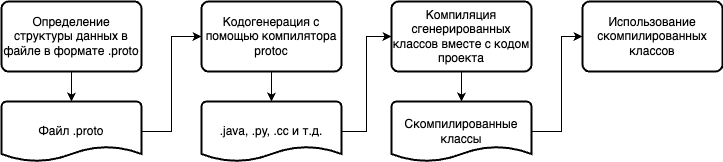
\includegraphics[width=0.85\linewidth]{\commonSecPathPrefix/sec_protobuf_sescription_attachments/protobuf_pipeline.drawio.png}
    \caption{Алгоритм работы разработчика с протоколом}
    \label{fig:protobuf_algo}
\end{figure}


Для начала разработчик описывает структуру передаваемых данных в файле в формате \textit{.proto}. 
Далее с помощью компилятора \textit{protoc} генерируются классы на соответствующем языке программирования, предоставляющие необходимые геттеры и сеттеры,
а также служебные методы для извлечения данных из файлов и потоков, извлечения отдельных значений из данных, 
проверки заполненности полей, сериализации данных обратно в файл или поток и других полезных функций.

\subsection{Формат описания сообщений в формате protobuf}

Единица данных, инкапсулирующая в себе данные о некоторой сущности, в протоколе protobuf называется 
сообщением и представляет собой аналог класса в языках программирования \cite{protobuf_api}.
Существует две версии формата описания protobuf-сообщений ~--~ \textit{proto2} и \textit{proto3}. Рассмотрим формат описания второй версии, а затем отдельно отметим отличия третьей версии.

Описание сообщения начинается с ключевого слова \textit{message}. Далее следует название сообщения, после в фигурных скобочках описываются поля сообщения, разделённые точкой с запятой.
В начале описания сообщения идёт ключевое слово \textit{optional} или \textit{required}, определяющее соттветственно является ли поле обязательным к заполнению или опциональным. В случае, если при парсинге обязательное поле не заполнено, будет выброшена ошибка. Далее следует указание типа данных поля. Тип данных может быть:
\begin{itemize}
    \item одним из примитивных типов, таких как целое число, число с плавающей точкой, логическое значение и т.д. Полный список примитивных типов, доступных в протоколе, представлен в таблице \ref{sec_proto_desc:table:fields_desc};
    \item другим сообщением, ранее определённым пользователем;
    \item перечислением (enum);
    \item типом \textit{oneof}, который представляет собой аналог \textit{union} языка С++;
    \item словарём.
\end{itemize}

\begin{longtable}{
    | >{\raggedright\arraybackslash}m{0.100\textwidth}
    | >{\raggedright\arraybackslash}m{0.100\textwidth}
    | >{\raggedright\arraybackslash}m{0.140\textwidth}
    | >{\raggedright\arraybackslash}m{0.120\textwidth}
    | >{\raggedright\arraybackslash}m{0.100\textwidth}
    | >{\raggedright\arraybackslash}m{0.120\textwidth}
    | >{\raggedright\arraybackslash}m{0.140\textwidth}
    |}
    
    \caption{Соответствие встроенных типов протокола Protocol buffers типам в популярных языках программирования}
    \label{sec_proto_desc:table:fields_desc} \\
    \hline
    \centering\arraybackslash Proto & 
    \centering\arraybackslash C++ & 
    \centering\arraybackslash Java / Kotlin & 
    \centering\arraybackslash Python & 
    \centering\arraybackslash Go & 
    \centering\arraybackslash Ruby & 
    \centering\arraybackslash C\# \\
    \hline
    \endfirsthead

    \continueTableCaption \\
    \hline
    \centering\arraybackslash Proto & 
    \centering\arraybackslash C++ & 
    \centering\arraybackslash Java / Kotlin & 
    \centering\arraybackslash Python & 
    \centering\arraybackslash Go & 
    \centering\arraybackslash Ruby & 
    \centering\arraybackslash C\# \\
    \hline
    \endhead

    double & double & double & float & float64 & Float & double \\
    \hline
    float & float & float & float & float32 & Float & float \\
    \hline
    int32 & int32 & int & int & int32 & Fixnum or Bignum & int \\
    \hline
    int64 & int64 & long & int / long[4] & int64 & Bignum & long \\
    \hline
    uint32 & uint32 & int[2] & int / long[4] & uint32 & Fixnum / Bignum & uint \\
    \hline
    uint64 & uint64 & long[2] & int / long[4] & uint64 & Bignum & ulong \\
    \hline
    sint32 & int32 & int & int & int32 & Fixnum / Bignum & int \\
    \hline
    sint64 & int64 & long & int / long[4] & int64 & Bignum & long \\
    \hline
    fixed32 & uint32 & int[2] & int / long[4] & uint32 & Fixnum / Bignum & uint \\
    \hline
    fixed64 & uint64 & long[2] & int / long[4] & uint64 & Bignum & ulong \\
    \hline
    sfixed32 & int32 & int & int & int32 & Fixnum / Bignum & int \\
    \hline
    sfixed64 & int64 & long & int / long[4] & int64 & Bignum & long \\
    \hline
    bool & bool & boolean & bool & bool & TrueClass / FalseClass & bool \\
    \hline
    string & string & String & str / unicode[5] & string & String & string \\
    \hline
    bytes & string & ByteString & str / bytes & []byte & String & ByteString \\
    \hline

\end{longtable}

После указания обязательности и выбора типа поля указывается имя поля. При указании имён полей следует учитывать следующие замечания:
\begin{itemize}
    \item иногда бывает трудно или даже невозможно изменить имена полей после того, как они были использованы в рабочей среде;
    \item имена полей не могут содержать дефис;
    \item стандартом рекомендуется использовать множественные имена для повторяющихся (\textit{repeated}) полей.
\end{itemize}

После присвоения имени полю присваивается номер поля. Номер поля представляет из себя целое число от 1 до 536870911.
Номера полей нельзя изменить или использовать повторно внутри того же сообщения в целях сохранения обратной совместимости.
Если поле удаляется из сообщения, следует следить за тем, чтобы его номер не переиспользовался для другого в дальнейшем, так как это также приведёт к обратной несовместимости.
После номера сообщения в квадратных скобочках могут быть указаны опции полей ~--~ служебная информация, влияющая на кодогенерацию. Например, указав опцию \textit{json\_name}, можно установить имя ключа, который должен быть использован при конвертации сообщения в формат JSON.

Одной из главных отличительных особенностей формата \textit{proto3} от \textit{proto2} является опциональность всех полей по умолчанию.
Таким образом, в \textit{proto3} описание поля начинается сразу с типа данных, минуя ключевые слова \textit{optional} или \textit{required}.
Остальные отличия в описании форматов не влияют на ход данной дипломной работы.

Пример объявления сообщения представлен в листинге \ref{code:proto_example}:

\begin{lstlisting}[style=CodeListing, label=code:proto_example, caption={Пример простейшего protobuf-сообщения}]
message Person {
  string name = 1;
  int32 id = 2;
}
\end{lstlisting}

\subsection{Формат для кодирования целочисленных данных varint}
Формат varint (variable-length integer) является ключевой частью протокола сериализации Protocol Buffers 
и используется для эффективного кодирования целых чисел переменной длины. За счет переменной длины он позволяет 
представлять как маленькие, так и большие значения в достаточно компактном виде.
Так, если число меньше 128, то оно будет занимать лишь 1 байт. Однако, числа близкие к максимально возможным, 
будут занимать больше места, чем в обычном формате.
Например, максимальное значение, которое можно сохранить в 8-ми байтах, в формате varint занимает 10 байт.
Проблема возникает с кодированием отрицательных чисел, ведь у любого малого по модулю отрицательного числа старший бит выставлен в единицу, а значит,
закодированное в формате varint значение всегда будет занимать максимально возможную длину, даже если между знаковым битом и следующим единичным битом 
большое количество нулевых бит. Эту проблему разработчики решили с помощью алгоритма шифрования знаковых чисел ZigZag. Его суть состоит в переносе знакового бита
из старшего в младший разряд. Результат кодирования алгоритмом ZigZag может быть выражен формулой \ref{sec_proto_desc:eq:zigzag}:

\begin{equation}
    \label{sec_proto_desc:eq:zigzag}
    encoded\_value = (value << 1) \oplus (value >> (N - 1)) \text{,}
\end{equation}
\begin{explanationx}
\item [где] $ value $ ~--~ кодируемое значение;
\item       $ N $ ~--~ количество бит в двоичной записи $ value $.
\end{explanationx}

Декодирование выполняется более сложным способом: выполняется исключающее ИЛИ над закодированным значением,
сдвинутым на 1 вправо для удаления знакового бита, и знаковым битом, полученным из закодированного числа,
спроецированным на все биты через умножение на максимальное значение для N разрядов.
Таким образом, знаковый бит переносится из младшего разряда в старший. Соответственно, для декодирования значения в алгоритме ZigZag можно использовать формулу \ref{sec_proto_desc:eq:zigzag_decode}:
\begin{gather}
    \label{sec_proto_desc:eq:zigzag_decode}
        value = ((encoded\_value \land 1) * MAX\_VALUE(N)) \oplus \nonumber\\
        \oplus (encoded\_value >> 1) \text{,}
\end{gather}
\begin{explanationx}
\item [где] $ MAX\_VALUE(N) $ ~--~ число с N разрядами, заполненными единицами (например, 0xffffffff при N=32).
\end{explanationx}

Рассмотрим шаги алгоритма кодирования в формат varint:

\begin{enumerate}
    \item двоичное представление исходного числа разбивается на группы по 7 бит;
    \item перед каждой группой добавляется единичный бит, если группа не последняя, и нулевой бит иначе;
    \item группы конкатенируются, образуя результат кодирования.
\end{enumerate}

Следовательно, алгоритм декодирования значения представляет из себя следующую последовательность операций:
// TODO: сделать блок-схемку

Все числовые значения, кроме fixed64, sfixed64 и double, в протоколе кодируются в формате varint.

\subsection{Алгоритм сериализации}

Рассмотрим сериализацию сообщений в протоколе на практическом примере. Объявим в файле \textit{addressbook.proto} 
структуру данных, представленную в листинге \ref{code:addressbook_proto}:

\begin{lstlisting}[style=CodeListing, label=code:addressbook_proto, caption={Protobuf-сообщения AddressBook и Person}]
syntax = "proto2";

message Person {
  optional string name = 1;
  optional int32 id = 2;
  optional string email = 3;

  enum PhoneType {
    MOBILE = 0;
    HOME = 1;
    WORK = 2;
  }

  message PhoneNumber {
    optional string number = 1;
    optional PhoneType type = 2 [default = HOME];
  }

  repeated PhoneNumber phones = 4;
}

message AddressBook {
  repeated Person people = 1;
}
\end{lstlisting}

Такая структура описывает адресную книгу, которая является списком контактов.
Контакт содержит в себе имя, идентификационный номер, адрес электронной почты и список номеров
телефона с разделением по типам номеров телефона (мобильный, домашний, рабочий).

Далее напишем небольшую утилиту на C++, осуществляющую работу с данными сообщениями. С её помощью можно заполнить поля телефонной книги вручную и сериализовать её в бинарном виде в файл для последующего анализа. Код утилиты представлен в листинге \ref{code:proto_utility}

\begin{lstlisting}[style=CodeListing, label=code:proto_utility, caption={Утилита для работы с protobuf-сообщениями}]
#include <iostream>
#include <fstream>
#include <string>

#include "addressbook.pb.h"

using namespace std;

#define READ_EXAMPLE 1
#define WRITE_EXAMPLE 2
#define TYPE_EXAMPLE WRITE_EXAMPLE

void PromptForAddress(tutorial::Person* person) {
    cout << "Enter person ID number: ";
    int id;
    cin >> id;
    person->set_id(id);
    cin.ignore(256, '\n');

    cout << "Enter name: ";
    getline(cin, *person->mutable_name());

    cout << "Enter email address (blank for none): ";
    string email;
    getline(cin, email);
    if (!email.empty()) {
        person->set_email(email);
    }

    while (true) {
        cout << "Enter a phone number (or leave blank to finish): ";
        string number;
        getline(cin, number);
        if (number.empty()) {
            break;
        }

        tutorial::Person::PhoneNumber* phone_number = person->add_phones();
        phone_number->set_number(number);

        cout << "Is this a mobile, home, or work phone? ";
        string type;
        getline(cin, type);
        if (type == "mobile") {
            phone_number->set_type(tutorial::Person::MOBILE);
        }
        else if (type == "home") {
            phone_number->set_type(tutorial::Person::HOME);
        }
        else if (type == "work") {
            phone_number->set_type(tutorial::Person::WORK);
        }
        else {
            cout << "Unknown phone type.  Using default." << endl;
        }
    }

}

void ListPeople(const tutorial::AddressBook& address_book) {
    for (int i = 0; i < address_book.people_size(); i++) {
        const tutorial::Person& person = address_book.people(i);

        cout << "Person ID: " << person.id() << endl;
        cout << "  Name: " << person.name() << endl;
        if (person.has_email()) {
            cout << "  E-mail address: " << person.email() << endl;
        }

        for (int j = 0; j < person.phones_size(); j++) {
            const tutorial::Person::PhoneNumber& phone_number = person.phones(j);

            switch (phone_number.type()) {
            case tutorial::Person::MOBILE:
                cout << "  Mobile phone #: ";
                break;
            case tutorial::Person::HOME:
                cout << "  Home phone #: ";
                break;
            case tutorial::Person::WORK:
                cout << "  Work phone #: ";
                break;
            }
            cout << phone_number.number() << endl;
        }
    }
}


int main(int argc, char* argv[]) {
    GOOGLE_PROTOBUF_VERIFY_VERSION;

    if (argc != 2) {
        cerr << "Usage:  " << argv[0] << " ADDRESS_BOOK_FILE" << endl;
        return -1;
    }

    tutorial::AddressBook address_book;

#if(TYPE_EXAMPLE == WRITE_EXAMPLE)
    {
        // Read the existing address book.
        fstream input(argv[1], ios::in | ios::binary);
        if (!input) {
            cout << argv[1] << ": File not found.  Creating a new file." << endl;
        }
        else if (!address_book.ParseFromIstream(&input)) {
            cerr << "Failed to parse address book." << endl;
            return -1;
        }
    }

    // Add an address.
    PromptForAddress(address_book.add_people());
    PromptForAddress(address_book.add_people());

    {
        // Write the new address book back to disk.
        fstream output(argv[1], ios::out | ios::trunc | ios::binary);
        if (!address_book.SerializeToOstream(&output)) {
            cerr << "Failed to write address book." << endl;
            return -1;
        }
    }

#elif(TYPE_EXAMPLE == READ_EXAMPLE)

    {
        // Read the existing address book.
        fstream input(argv[1], ios::in | ios::binary);
        if (!address_book.ParseFromIstream(&input)) {
            cerr << "Failed to parse address book." << endl;
            return -1;
        }
    }

    ListPeople(address_book);

#endif
    // Optional:  Delete all global objects allocated by libprotobuf.
    google::protobuf::ShutdownProtobufLibrary();

    return 0;
}
\end{lstlisting}

Запустим программу и заполним телефонную книгу двумя контактами:

\begin{lstlisting}[style=CodeListing]
Enter person ID number: 170
Enter name: name1
Enter email address (blank for none): mail1
Enter a phone number (or leave blank to finish): 1234567
Is this a mobile, home, or work phone? mobile
Enter a phone number (or leave blank to finish):
Enter person ID number: 85
Enter name: name2
Enter email address (blank for none): mail2
Enter a phone number (or leave blank to finish): 7654321
Is this a mobile, home, or work phone? mobile
Enter a phone number (or leave blank to finish):
\end{lstlisting}

Идентификаторы, равные 170 и 85 выбраны для удобства: в шестнадцатиричном представлении они выглядят как \textit{AA} и \textit{55} соответственно, что облегчает просмотр бинарных данных.
Рассмотрим получившееся бинарное представление:

В результате работы программы получим бинарное представление, представленное на рисунке \ref{fig:encoded_proto}
\begin{figure}[ht]
    \centering
    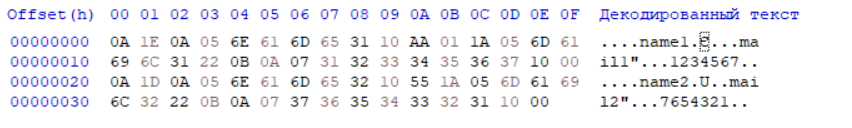
\includegraphics[width=0.85\linewidth]{\commonSecPathPrefix/sec_protobuf_sescription_attachments/encoded_proto.png}
    \caption{Сериализованное сообщение}
    \label{fig:encoded_proto}
\end{figure}

В protobuf данные хранятся по принципу ключ-значение. Ключ определяется по формуле \ref{sec_proto_desc:eq:proto_key}:
\begin{equation}
    \label{sec_proto_desc:eq:proto_key}
    (fieldNumber << 3) \lor wireType
\end{equation}
\begin{explanationx}
\item [где] $ fieldNumber $ ~--~ номер у переменной в описании структуры данных в файле *.proto;
\item       $ wireType $ ~--~ значение, определяемое таблицей \ref{sec_proto_desc:table:wire_type_value}.
\end{explanationx}
\begin{longtable}{
    | >{\raggedright\arraybackslash}m{0.300\textwidth}
    | >{\raggedright\arraybackslash}m{0.300\textwidth}
    | >{\raggedright\arraybackslash}m{0.315\textwidth}
    |}
    
    \caption{Определение значения wireType}
    \label{sec_proto_desc:table:wire_type_value} \\
    \hline
    \centering\arraybackslash Значение wireType & 
    \centering\arraybackslash Описание данных & 
    \centering\arraybackslash Используется для типов \\
    \hline
    \endfirsthead

    \continueTableCaption \\
    \hline
    \centering\arraybackslash Значение wireType & 
    \centering\arraybackslash Описание данных & 
    \centering\arraybackslash Используется для типов \\
    \hline
    \endhead

    0 & Varint & int32, int64, uint32, uint64, sint32, sint64, bool, enum \\
    \hline
    1 & 64-битная переменная & fixed64, sfixed64, double \\
    \hline
    2 & Переменная длина & string, bytes, вложенные сообщения, repeated-поля \\
    \hline
    3 & Устаревшее, не используется & - \\
    \hline
    4 & Устаревшее, не используется & - \\
    \hline
    5 & 32-битная переменная & fixed32, sfixed32, float \\
    \hline

\end{longtable}

Воспользовавшись формулой \ref{sec_proto_desc:eq:proto_key} определим, какой ключ должен быть перед переменной id:
\begin{equation*}
    key = 2 << 3 \lor 0 = 0x10
\end{equation*}

Это же число видим в декодированом файле.

Определим ключ для переменной name типа string, воспользовавшись формулой \ref{sec_proto_desc:eq:proto_key}: 
\begin{equation*}
    1 << 3 \lor 2 = 0x0A
\end{equation*}

Заметим, что перед переменными name1 и name2 (0x04 и 0x24 байт) стоит не 0x0A а 0x05. Это основная особенность типов с переменной длиной. Для таких типов идёт сначала ключ, потом количество байт. 0x05 описывает количество байт на данную переменную. 


